\chapter{Singular Value Decomposition}
\label{chap:SingularValueDecomposition}

We will picture the action of linear maps.
Specifically, we will draw 
the action of linear transformations $\map{h}{\Re^2}{\Re^2}$.
That will connect with an important way to factor matrices, and lead to
an interesting application.


\section{Drawing the action}
A defining property of linear maps is that 
$h(r\cdot\vec{v})=r\cdot h(\vec{v})$.
Recall that a line through the origin in $\Re^n$ has the form 
$\set{r\cdot \vec{v}\suchthat r\in\Re}$ for some~$\vec{v}\in\Re^n$. 
Thus the scalar multiplication property  
imposes a uniformity condition on a linear map:~its action on any 
line through the origin is determined by its action
on any nonzero vector in that line.

For instance, consider the line~$y=2x$ in the plane
\begin{equation*}
  \set{r\cdot\colvec{1 \\ 2}\suchthat r\in\Re}
\end{equation*}
and suppose that $\map{t}{\Re^2}{\Re^2}$ is represented by this matrix.
\begin{equation*}
  \rep{t}{\stdbasis_2,\stdbasis_2}
  =
  \begin{mat}
    1 &2 \\
    3 &4
  \end{mat}
\end{equation*}
Then the map $t$ has this effect on one of the line's vectors.
\begin{equation*}
  \vec{v}=\colvec{1 \\ 2}\mapsunder{t}\colvec{5 \\ 11}
\end{equation*}
On $2\vec{v}$ the 
map has twice the effect, on  $3\vec{v}$ it has three times the
effect, etc.
\begin{equation*}
  \colvec{2 \\ 4}\mapsunder{t}\colvec{10 \\ 22}
  \qquad
  \colvec{3 \\ 6}\mapsunder{t}\colvec{15 \\ 33}
  \qquad
  \colvec{r \\ 2r}\mapsunder{t}\colvec{5r \\ 11r}
\end{equation*}
We can use this observation to show the action of 
linear transformations of the plane, $\map{t}{\Re^2}{\Re^2}$
(we choose the plane simply because the pictures are 
easy to draw and to understand). 

The $t(r\cdot\vec{v})=r\cdot t(\vec{v})$ relationship says that
a linear map has the same effect on all vectors in a line through the
origin.
So to picture a transformation's action we will fix 
one nonzero vector~$\vec{v}$ from each line through the origin,
and show where the transformation $t(\vec{v})$ takes it.
The natural set containing one point from each line through the origin 
is the upper half of the unit circle, shown here
(the colors are explained below).
% \begin{sagecommandline}
% sage: load("plot_action.sage")
% sage: p = plot_circle_action(1,0,0,1) 
% sage: p.set_axes_range(-1.5, 1.5, -0.5, 1.5) 
% sage: p.save("graphics/svd000.pdf")
% \end{sagecommandline}
\begin{sagesilent}
load("plot_action.sage")
p = plot_circle_action(1,0,0,1) 
p.set_axes_range(-1.5, 1.5, -0.5, 1.5) 
p.save("graphics/svd000.pdf")
\end{sagesilent}
\begin{equation*}
  U=\set{\vec{v}=\colvec{\cos(t) \\ \sin(t)}
         \suchthat 
         0\leq t<\pi}
  \qquad
  \vcenteredhbox{\includegraphics{graphics/svd000.pdf}}  
\end{equation*}
The point $(1,0)$ is included in that set, as the representative of
the $x$~axis, but
$(-1,0)$ is not, which is why that point has an open circle.

The first illustration is for a simple transformation.
\begin{equation*}
  \colvec{x \\ y} \mapsto \colvec{2x \\ y}
\end{equation*}
\Sage{} can compute the effect of this transformation
on the upper half circle. 
The code below inputs the file \inlinecode{plot_action.sage}
to get access to the routine
\inlinecode{plot_circle_action(a,b,c,d)}. 
This divides the input upper half circle into a number of curved segments,
the red one, the orange one, etc., then it 
multiplies the points on those curved segments 
by this matrix
\begin{equation*}
  \begin{mat}
    a &b \\
    c &d
  \end{mat}
\end{equation*}
and finally it connects those output segments to get an output curve, where 
the output segments are colored red, orange, etc.
The listing of the full source of \inlinecode{plot_action.sage} is 
at the end of this chapter.
\begin{sagecommandline}
sage: load("plot_action.sage")
sage: q = plot_circle_action(1,0,0,1) 
sage: q.set_axes_range(-2, 2, -1, 2) 
sage: q.save("graphics/svd001a.pdf")
sage: p = plot_circle_action(2,0,0,1) 
sage: p.set_axes_range(-2, 2, -1, 2) 
sage: p.save("graphics/svd001b.pdf")
\end{sagecommandline}
% \begin{sagesilent}
% load("plot_action.sage")
% q = plot_circle_action(1,0,0,1) 
% q.set_axes_range(-2, 2, -1, 2) 
% q.save("graphics/svd001a.pdf")
% p = plot_circle_action(2,0,0,1) 
% p.set_axes_range(-2, 2, -1, 2) 
% p.save("graphics/svd001b.pdf")
% \end{sagesilent}
Here is the before and after, the upper half circle 
and the associated output.
The colors show the association\Dash which of the 
points on the left are mapped to which of the points 
on the right.
\begin{equation*}
  \vcenteredhbox{\includegraphics{graphics/svd001a.pdf}}
  \quad\mapsunder{\big (\begin{smallmatrix} 2 &0 \\ 0 &1 \end{smallmatrix}\big )}\quad
  \vcenteredhbox{\includegraphics{graphics/svd001b.pdf}}
\end{equation*}
\Sage{} drew the unit circle by plotting the action of the identity map.
Then \Sage{} drew the effect of the transformation by plotting the
action of this matrix.
\begin{equation*}
\begin{mat}
  2  &0  \\
  0  &1
\end{mat}
\end{equation*}

The next before and after picture shows
the effect of the map
\begin{equation*}
  \colvec{x \\ y} \mapsto \colvec{-x \\ 3y}
\end{equation*}
that triples the $y$~component and also multiplies the 
$x$~component by $-1$.\footnote{%
  As in other chapters, some of the graphics are drawn using 
  some options that are not shown.
  In this case, the two \protect\inlinecode{p.save(...)} commands have
  the \protect\inlinecode{ticks\_integer=True} option.
  Not showing these options just reduces clutter that isn't linear algebra.}
\begin{sagecommandline}
sage: q = plot_circle_action(1,0,0,1) 
sage: q.set_axes_range(-2, 2, -1.25, 3.25) 
sage: q.save("graphics/svd002a.pdf")
sage: p = plot_circle_action(-1,0,0,3) 
sage: p.set_axes_range(-2, 2, -1.25, 3.25) 
sage: p.save("graphics/svd002b.pdf")
\end{sagecommandline}
\begin{sagesilent}
load("plot_action.sage")
q = plot_circle_action(1,0,0,1) 
q.set_axes_range(-2, 2, -1.25, 3.25) 
q.save("graphics/svd002a.pdf", ticks_integer=True)
p = plot_circle_action(-1,0,0,3) 
p.set_axes_range(-2, 2, -1.25, 3.25) 
p.save("graphics/svd002b.pdf", ticks_integer=True)
\end{sagesilent}
\begin{equation*}
  \vcenteredhbox{\includegraphics{graphics/svd002a.pdf}}
  \quad\mapsunder{\big (\begin{smallmatrix} -1 &0 \\ 0 &3 \end{smallmatrix}\big )}\quad
  \vcenteredhbox{\includegraphics{graphics/svd002b.pdf}}
\end{equation*}
Tripling the $y$ component is easy to understand.
As for taking the negative of the $x$ component, 
this is where the colors have something to say.
On the input circle, when you move counterclockwise, the colors go from 
red to orange, to green, blue, indigo, and then violet.
But the output does the opposite:~moving counterclockwise it
passes from violet to red.
This transformation changes the orientation,
or `sense', of the curve. 

This is rotation by $\pi/4$~radians, clockwise.
\begin{equation*}
  \colvec{x \\ y} \mapsto \colvec{\cos(-\pi/4)-\sin(-\pi/4) \\ \sin(-\pi/4)+\cos(-\pi/4)}
\end{equation*}
\begin{sagecommandline}
sage: q = plot_circle_action(1,0,0,1) 
sage: q.set_axes_range(-1.5, 1.5, -1, 1.5) 
sage: q.save("graphics/svd003a.pdf")
sage: p = plot_circle_action(cos(-pi/4),-sin(-pi/4),sin(-pi/4),cos(-pi/4)) 
sage: p.set_axes_range(-1.5, 1.5, -1, 1.5) 
sage: p.save("graphics/svd003b.pdf")
\end{sagecommandline}
\begin{equation*}
  \vcenteredhbox{\includegraphics{graphics/svd003a.pdf}}
  \quad\mapsunder{\big (\begin{smallmatrix} \cos(-\pi/4) &-\sin(-\pi/4) \\ \sin(-\pi/4) &\cos(-\pi/4) \end{smallmatrix}\big )}\quad
  \vcenteredhbox{\includegraphics{graphics/svd003b.pdf}}
\end{equation*}

The next transformation is a shear.\footnote{%
  The definition from physics or engineering is that a shear is the motion of 
  two parts of a body where they slide   
  relative to each other in a direction parallel to their 
  plane of contact.  
  Thus, when you write with a pencil the flakes of
  graphite shear off on the paper.}
\begin{equation*}
  \colvec{x \\ y} \mapsto \colvec{x+2y \\ y}
\end{equation*}
Here, the first component of the output is affected
by the input's distance from the $y$-axis.
Input vectors higher up in the picture have their first component affected more
than do input vectors near the $x$-axis.
\begin{sagecommandline}
sage: q = plot_circle_action(1,0,0,1) 
sage: q.set_axes_range(-1.5, 2.5, -.25, 1.25) 
sage: q.save("graphics/svd004a.pdf")
sage: p = plot_circle_action(1,2,0,1) 
sage: p.set_axes_range(-1.5, 2.5, -.25, 1.25) 
sage: p.save("graphics/svd004b.pdf")
\end{sagecommandline}
\begin{sagesilent}
load("plot_action.sage")
q = plot_circle_action(1,0,0,1) 
q.set_axes_range(-1.5, 2.5, -.25, 2.25) 
q.save("graphics/svd004a.pdf", ticks_integer=True)
p = plot_circle_action(1,2,0,1) 
p.set_axes_range(-1.5, 2.5, -.25, 2.25) 
p.save("graphics/svd004b.pdf", ticks_integer=True)
\end{sagesilent}
\begin{equation*}
  \vcenteredhbox{\includegraphics{graphics/svd004a.pdf}}
  \quad\mapsunder{\big (\begin{smallmatrix} 1 &2 \\ 0 &1 \end{smallmatrix}\big )}\quad
  \vcenteredhbox{\includegraphics{graphics/svd004b.pdf}}
\end{equation*}

Next is a shear
where it is the output's 
second component that is is affected,
here by the input's distance from 
the $x$-axis.
\begin{equation*}
  \colvec{x \\ y} \mapsto \colvec{x \\ (1/2)x+y}
\end{equation*}
\begin{sagecommandline}
sage: q = plot_circle_action(1,0,0,1) 
sage: q.set_axes_range(-1.25, 1.25, -0.75, 1.5) 
sage: q.save("graphics/svd005a.pdf")
sage: p = plot_circle_action(1,0,1/2,1) 
sage: p.set_axes_range(-1.25, 1.25, -0.75, 1.5) 
sage: p.save("graphics/svd005b.pdf")
\end{sagecommandline}
% \begin{sagesilent}
% load("plot_action.sage")
% q = plot_circle_action(1,0,0,1) 
% q.set_axes_range(-2, 2, -2, 2) 
% q.save("graphics/svd005a.pdf")
% p = plot_circle_action(1,0,1/2,1) 
% p.set_axes_range(-2, 2, -2, 2) 
% p.save("graphics/svd005b.pdf")
% \end{sagesilent}
\begin{equation*}
  \vcenteredhbox{\includegraphics{graphics/svd005a.pdf}}
  \quad\mapsunder{\big (\begin{smallmatrix} 1 &0 \\ 1/2 &1 \end{smallmatrix}\big )}\quad
  \vcenteredhbox{\includegraphics{graphics/svd005b.pdf}}
\end{equation*}

And here is a generic transformation.
It changes orientation also.
\begin{sagecommandline}
sage: q = plot_circle_action(1,0,0,1) 
sage: q.set_axes_range(-2, 4, -3, 6) 
sage: q.save("graphics/svd006a.pdf")
sage: p = plot_circle_action(1,2,3,4) 
sage: p.set_axes_range(-2, 4, -3, 6) 
sage: p.save("graphics/svd006b.pdf")
\end{sagecommandline}
% \begin{sagesilent}
% load("plot_action.sage")
% q = plot_circle_action(1,0,0,1) 
% q.set_axes_range(-2, 4, -3, 6) 
% q.save("graphics/svd006a.pdf",figsize=3)
% p = plot_circle_action(1,2,3,4) 
% p.set_axes_range(-2, 4, -3, 6) 
% p.save("graphics/svd006b.pdf",figsize=3)
% \end{sagesilent}
\begin{equation*}
  \vcenteredhbox{\includegraphics{graphics/svd006a.pdf}}
  \quad\mapsunder{\big (\begin{smallmatrix} 1 &2 \\ 3 &4 \end{smallmatrix}\big )}\quad
  \vcenteredhbox{\includegraphics{graphics/svd006b.pdf}}
\end{equation*}



\section{SVD}
In those pictures the image of the unit circle is an ellipse.
Recall that in $\Re^2$ an ellipse has a major axis, 
the longer one, and a minor axis.\footnote{%
  If the two axes have the same length,
  as in the output of the rotation map, 
  then the ellipse is a circle.
  If one axis has length zero then the ellipse is a line segment 
  and if both have length zero then it is a point.}
Write $\sigma_1$ for the length of the semi-major axis, 
the distance from the center to the furthest-away point on the ellipse,
and write $\sigma_2$ for the length of the semi-minor axis.
\begin{sagecommandline}
sage: plot.options['axes_pad'] = 0.5
sage: plot.options['fontsize'] = 4
sage: plot.options['aspect_ratio'] = 1
sage: sigma_1=3
sage: sigma_2=1
sage: E = ellipse((0,0), sigma_1, sigma_2)
sage: E.save("graphics/svd100.pdf")
\end{sagecommandline}
\begin{sagesilent}
plot.options['axes_pad'] = 0.5
plot.options['fontsize'] = 2
plot.options['aspect_ratio'] = 1
plot.options['figsize'] = 1
sigma_1=3
sigma_2=1
E = ellipse((0,0), sigma_1, sigma_2)
# E.save("graphics/svd100.pdf", axes_pad=0.075, dpi=1200, fontsize=7, ticks=([-3,-2,-1,1,2,3],[-1,1]), figsize=1.5)
E.save("graphics/svd100.pdf", ticks_integer=True, axes_pad=0.075, figsize=3)
\end{sagesilent}
\begin{center}
  \includegraphics{graphics/svd100.pdf}
\end{center}
The two are orthogonal.
Above, the major axis is on the $x$-axis while the
minor is on the $y$-axis.

Under any linear map $\map{t}{\Re^n}{\Re^m}$ the 
unit sphere maps to a hyperellipse.
This is a version of the \textit{Singular Value Decomposition} of
matrices:
for any linear map $\map{t}{\Re^n}{\Re^m}$ there are bases
$B=\sequence{\vec{\beta}_1,\ldots,\vec{\beta}_n}$ for the domain and
$D=\sequence{\vec{\delta}_1,\ldots,\vec{\delta}_m}$ for the codomain
such that $t(\vec{\beta}_i)=\sigma_i\vec{\delta}_i$ (for $i\leq n$), where the
scalars $\sigma_i$ are called \textit{singular values}.
The next section sketches a proof
but we first illustrate this result by using an example matrix.
\Sage{} will find the two bases $B$ and~$D$ and will picture how the 
vectors $\vec{\beta}_i$ 
are mapped to the $\sigma_i\vec{\delta}_i$.

So consider again the generic matrix.
Here is its action again, shown
on a full circle.
\begin{sagecommandline}
sage: load("plot_action.sage")
sage: q = plot_circle_action(1,0,0,1,full_circle=True) 
sage: q.set_axes_range(-3, 3, -5, 5) 
sage: q.save("graphics/svd101a.pdf")
sage: p = plot_circle_action(1,2,3,4,full_circle=True) 
sage: p.set_axes_range(-3, 3, -5, 5) 
sage: p.save("graphics/svd101b.pdf")
\end{sagecommandline}
\begin{sagesilent}
load("plot_action.sage")
q = plot_circle_action(1,0,0,1,full_circle=True) 
q.set_axes_range(-3, 3, -5, 5) 
q.save("graphics/svd101a.pdf", ticks_integer=True)
p = plot_circle_action(1,2,3,4,full_circle=True) 
p.set_axes_range(-3, 3, -5, 5) 
p.save("graphics/svd101b.pdf", ticks_integer=True)
\end{sagesilent}
\begin{equation*}
  \vcenteredhbox{\includegraphics{graphics/svd101a.pdf}}
  \quad\mapsunder{\big (\begin{smallmatrix} 1 &2 \\ 3 &4 \end{smallmatrix}\big )}\quad
  \vcenteredhbox{\includegraphics{graphics/svd101b.pdf}}
  \tag{$*$}
\end{equation*}
\Sage{} will find the SVD of this example matrix.
\begin{sagecommandline}
sage: M = matrix(RDF, [[1, 2], [3, 4]])
sage: U,Sigma,V = M.SVD()
sage: U
sage: Sigma
sage: V
sage: U*Sigma*(V.transpose())
\end{sagecommandline}
\noindent 
The Singular Value Decomposition has $M$ as the product of
three matrices, $U\Sigma\trans{V}$.
The basis vectors $\vec{\beta}_1$, $\vec{\beta}_2$, $\vec{\delta}_1$, 
and~$\vec{\delta}_2$ are the columns of $U$ and~$V$. 
The singular values are the diagonal entries of~$\Sigma$.
\Sage{} will plot the effect of the transformation
on the basis vectors for the domain so we can compare those with the
basis vectors for the codomain.
\begin{sagecommandline}
sage: M = matrix(RDF, [[1, 2], [3, 4]])
sage: U,Sigma,V = M.SVD()
sage: beta_1 = vector(RDF, [U[0][0], U[1][0]])
sage: beta_2 = vector(RDF, [U[0][1], U[1][1]])
sage: delta_1 = vector(RDF, [V[0][0], V[1][0]])
sage: delta_2 = vector(RDF, [V[0][1], V[1][1]])
sage: C = circle((0,0), 1)
sage: P = C + plot(beta_1) + plot(beta_2)
sage: P.save("graphics/svd102a.pdf")
sage: image_color=Color(1,0.5,0.5)   # color for t(beta_1), t(beta_2)
sage: Q = C + plot(beta_1*M, width=3) 
sage: Q = Q + plot(delta_1,width=1.4) 
sage: Q = Q + plot(beta_2*M,width=3) 
sage: Q = Q + plot(delta_2,width=1.4)
sage: Q.save("graphics/svd102b.pdf")
\end{sagecommandline}
\begin{sagesilent}
M = matrix(RDF, [[1, 2], [3, 4]])
U,Sigma,V = M.SVD()
beta_1 = vector(RDF, [U[0][0], U[1][0]])
beta_2 = vector(RDF, [U[0][1], U[1][1]])
delta_1 = vector(RDF, [V[0][0], V[1][0]])
delta_2 = vector(RDF, [V[0][1], V[1][1]])
plot.options['axes_pad'] = 0.05
plot.options['fontsize'] = 7
plot.options['aspect_ratio'] = 1
s = 2  # uniform arrowsize
C = circle((0,0), 1)
P = C + plot(beta_1,arrowsize=s) + plot(beta_2,arrowsize=s)
P.save("graphics/svd102a.pdf",figsize=2, ticks_integer=True)
image_color=Color(1,0.5,0.5)   # color for t(beta_1), t(beta_2)
Q = C + plot(beta_1*M, width=3,color=image_color,arrowsize=s) 
Q = Q + plot(delta_1,width=1.4,color='blue',arrowsize=s) 
Q = Q + plot(beta_2*M,width=3,color=image_color,arrowsize=s) 
Q = Q + plot(delta_2,width=1.4,color='blue',arrowsize=s)
Q.save("graphics/svd102b.pdf",figsize=4.467, ticks_integer=True)
\end{sagesilent}
Below, the domain's 
blue $\vec{\beta}$'s on the left map to the codomain's light red 
$t(\vec{\beta})$'s on the right.
Also on the right, in blue, are the $\vec{\delta}$'s.
The diagonal entries of $\Sigma$ tell us about the
red vectors:~$t(\vec{\beta}_1)$ is about $5.5$ times $\vec{\delta}_1$
while $t(\vec{\beta}_2)$ is about $0.4$ times~$\vec{\delta}_2$.
\begin{equation*}
  % \setlength{\fboxsep}{0in} % used to set box heights by eye; surrounded each picture env with a fbox
  \setlength{\unitlength}{1in}
  \begin{picture}(1.35,1.35)
    \put(0,1.825){\includegraphics{graphics/svd102a.pdf}}
    \put(.3,1.9){\scriptsize $\vec{\beta}_1$}
    \put(0,2.7){\scriptsize $\vec{\beta}_2$}
  \end{picture}
  \quad
  \raisebox{2.65in}{$\mapsunder{\big (\begin{smallmatrix} 1 &2 \\ 3 &4 \end{smallmatrix}\big )}$}
  \qquad
  \begin{picture}(2.45,3.15)
    \put(0,0){\includegraphics{graphics/svd102b.pdf}}
    \put(1.25,2){\scriptsize $\vec{\delta}_1$}
    \put(2.3,2.1){\scriptsize $\vec{\delta}_2$}
  \end{picture}
  \tag*{\raisebox{2.5in}{($**$)}}
\end{equation*}
The two bases are orthonormal,
comprised of unit vectors that are orthogonal.
Note also, by comparing with the diagram above labeled~($*$), that
long red vector is the
semi-major axis while its short red vector is the  
semi-minor axis.



\section{Proof sketch}

Consider an~$\nbyn{n}$ matrix~$T$ that is nonsingular.
Let $\map{t}{\Re^n}{\Re^n}$ be the
nonsingular transformation represented by
$T$ with respect to the standard bases.
We will argue that there are scalars $\sigma_0$, \ldots~$\sigma_n$
and bases
$B=\sequence{\vec{\beta}_1,\ldots,\vec{\beta}_n}$ and
$D=\sequence{\vec{\delta}_1,\ldots,\vec{\delta}_n}$ for the 
domain and codomain
such that $t(\vec{\beta}_i)=\sigma_i\vec{\delta}_i.$\footnote{%
  This argument, 
  from \protect\cite{BlankKrikorianSpring89},
  is a sketch because it uses results that a reader may have seen only 
  seen only in a form not as strong as needed by the theorem, 
  and because it relies on material from the book that is optional.
  In addition, we'll consider only the case of a nonsingular matrix and map.
  This gives the main idea, which is the point of a sketch.}

Recall Calculus~I's Extreme Value Theorem: for a continuous
function~$f$, if a subset $D\subset \Re$ of the real line 
is closed and bounded then
its image $f(D)=\set{f(d)\suchthat d\in D}$ 
is also closed and bounded (see \cite{wiki:ExtremeValueThm}).
A generalization of that result gives that because the unit sphere in $\Re^n$
is closed and bounded then its image under~$t$ is closed and bounded.
Although we won't prove this, the image is a hyperellipse
so we will call it that. 

Because this hyperellipse is closed and bounded it has a 
point furthest from the origin (if it has more than one then just pick one).
Let $\vec{w}$ be a vector extending from the origin to that furthest point.
Let $\vec{v}$ be the member of the unit sphere that maps to $\vec{w}$.
Let $P$ be the plane tangent to the sphere at the endpoint of $\vec{v}$.
Let $Q$ be the image of $P$ under~$t$.
Since $t$ is one-to-one, $Q$ touches the ellipsoid only at~$\vec{w}$.
\begin{center}
  \includegraphics{asy/ellipsoid1.pdf}
\end{center}

As the illustration suggests, if we slide~$P$ along the 
vector~$\vec{v}$ to
the origin then the result is 
the subspace of $\Re^n$ of vectors perpendicular
to~$\vec{v}$.
This subspace has dimension~$n-1$. 
We will argue in the next paragraph 
that similarly $Q$ contains only
vectors perpendicular to~$\vec{w}$.
With that we can complete an argument by induction:~we 
start constructing the 
bases~$B$ and~$D$ by taking $\vec{\beta}_1$ to be~$\vec{v}$, taking
$\sigma_1$ to be the length $\norm{\vec{w}}$, and taking
$\vec{\delta}_1$ to be $\vec{w}/\norm{\vec{w}}$.
Then induction proceeds by taking the restriction of $t$ to~$P$.

Therefore consider~$Q$.
The plane that touches the ellipsoid
only at~$\vec{w}$ is unique since if there were another then its inverse image
under $t$
would be a second plane, besides~$P$, 
that touches the sphere only at~$\vec{v}$, which is impossible (since it is a
sphere).
To see that $Q$ is perpendicular to~$\vec{w}$ consider a sphere in the codomain
centered at the origin whose radius is the length, $\norm{\vec{w}}$.
This sphere has a plane tangent at the endpoint of~$\vec{w}$ 
that is perpendicular
to $\vec{w}$.
Because $\vec{w}$ ends at a point on the ellipsoid furthest from the origin,
the ellipsoid is entirely contained in this sphere, so its tangent plane 
touches the ellipsoid only at~$\vec{w}$.
Therefore
this tangent plane is~$Q$. 
That ends the argument.



\section{Matrix factorization}

We can express those geometric ideas in an algebraic form
(for a proof see \cite{TrefethenBau97}).

The \textit{singular value decomposition} of an $\nbym{m}{n}$ matrix~$A$
is a factorization, $A=U\Sigma \trans{V}$\!.
The $\nbym{m}{n}$ matrix $\Sigma$ 
is all zeroes except for diagonal entries, the singular values, 
$\sigma_1\geq \sigma_2 \geq \cdots \geq \sigma_r> 0$ where $r$ is the
rank of~$A$.
The $\nbyn{m}$ matrix~$U$ and the $\nbyn{n}$ matrix~$V$ are unitary, meaning
that their columns form an orthogonal basis of unit vectors, called 
the left and 
right singular vectors for~$A$. 
\begin{sagecommandline}
sage: M = matrix(RDF, [[0, 1, 2], [3, 4, 5]])
sage: U,Sigma,V = M.SVD()
sage: U
sage: Sigma
sage: V  
\end{sagecommandline}
The number of singular values is the row rank of the matrix.
Here \Sage{} gets a $\sigma_2$ that is not quite \( 1 \) because of numerical 
issues. 
% \begin{sagecommandline}
% sage: M = matrix(RDF, [[0, 1, 2], [0, 2, 4]])
% sage: U,Sigma,V = M.SVD()
% sage: U
% sage: Sigma
% sage: V  
% \end{sagecommandline}

The product $U\Sigma\trans{V}$ simplifies.
For instance, 
consider the case where all three matrices are $\nbyn{2}$.
Write $\vec{u}_1$, $\vec{u}_2$ for the columns of~$U$
and $\vec{v}_1$, $\vec{v_2}$ for the columns of~$V$,
so that the rows of $\trans{V}$ are $\trans{\vec{v}}_1$ and
$\trans{\vec{v}}_2$.
\begin{align*}
  U\Sigma \trans{V}
  &=
  \begin{mat}
    \vec{u}_1 &\vec{u}_2
  \end{mat}
  \begin{mat}
    \sigma_1 &0 \\
    0        &\sigma_2
  \end{mat}
  \begin{mat}
    \trans{\vec{v}}_1 \\[.75ex]
    \trans{\vec{v}}_2
  \end{mat}             % \\[.5ex]
  =
  \begin{mat}
    \vec{u}_1 &\vec{u}_2
  \end{mat}
  \,[
  \begin{mat}
    \sigma_1 &0 \\
    0        &0
  \end{mat}
  +
  \begin{mat}
    0 &0 \\
    0        &\sigma_2
  \end{mat}
  ]\,
  \begin{mat}
    \trans{\vec{v}}_1 \\[.75ex]
    \trans{\vec{v}}_2
  \end{mat}             \\[.5ex]
  &=
  \begin{mat}
    \vec{u}_1 &\vec{u}_2
  \end{mat}
  \begin{mat}
    \sigma_1 &0 \\
    0        &0
  \end{mat}
  \begin{mat}
    \trans{\vec{v}}_1 \\[.75ex]
    \trans{\vec{v}}_2
  \end{mat}             
  +
  \begin{mat}
    \vec{u}_1 &\vec{u}_2
  \end{mat}
  \begin{mat}
    0        &0 \\
    0        &\sigma_2
  \end{mat}
  \begin{mat}
    \trans{\vec{v}}_1 \\[.75ex]
    \trans{\vec{v}}_2
  \end{mat}             \\[.5ex]
  &=
  \sigma_1\cdot
  \begin{mat}
    \vec{u}_1 &\vec{u}_2
  \end{mat}
  \begin{mat}
    1 &0 \\
    0 &0
  \end{mat}
  \begin{mat}
    \trans{\vec{v}}_1 \\[.75ex]
    \trans{\vec{v}}_2
  \end{mat}             
  +
  \sigma_2\cdot 
  \begin{mat}
    \vec{u}_1 &\vec{u}_2
  \end{mat}
  \begin{mat}
    0        &0 \\
    0        &1
  \end{mat}
  \begin{mat}
    \trans{\vec{v}}_1 \\[.75ex]
    \trans{\vec{v}}_2
  \end{mat}
  \tag{$*{*}*$}
\end{align*}
In the first term,
right multiplication by the $1,1$~unit matrix picks out the first column of
$U$, and left multiplication by the $1,1$~unit matrix picks out first row of
$V$ so those are the only parts that remain after the product.
In short, we get this.
\begin{equation*}
  \begin{mat}
    u_{1,1} &u_{1,2} \\
    u_{2,1} &u_{2,2}
  \end{mat}
  \begin{mat}
    1 &0 \\
    0 &0
  \end{mat}
  \begin{mat}
    v_{1,1} &v_{2,1} \\
    v_{1,2} &v_{2,2}
  \end{mat}
  =
  \begin{mat}
    u_{1,1}v_{1,1} &u_{1,1}v_{2,1} \\
    u_{2,1}v_{1,1} &u_{2,1}v_{2,1}
  \end{mat}
  =\colvec{u_{1,1} \\ u_{2,1}}\rowvec{v_{1,1} &v_{2,1}}
  =\vec{u}_1\trans{\vec{v}}_1
\end{equation*}
The second term simplifies in the same way.
\begin{equation*}
  \begin{mat}
    u_{1,1} &u_{1,2} \\
    u_{2,1} &u_{2,2}
  \end{mat}
  \begin{mat}
    0 &0 \\
    0 &1
  \end{mat}
  \begin{mat}
    v_{1,1} &v_{2,1} \\
    v_{1,2} &v_{2,2}
  \end{mat}
  =
  \begin{mat}
    u_{1,2}v_{1,2} &u_{1,2}v_{2,2} \\
    u_{2,2}v_{1,2} &u_{2,2}v_{2,2}
  \end{mat}
  =\vec{u}_2\trans{\vec{v}}_2
\end{equation*}
Thus, equation~($*{*}*$) simplifies to
$U\Sigma \trans{V}=\sigma_1\cdot\vec{u}_1\trans{\vec{v}}_1
   +\sigma_2\cdot\vec{u}_2\trans{\vec{v}}_2$.
Cases other than~$\nbyn{2}$ work the same way.



\section{Application: data compression}

We can write any matrix as a sum
$M=\sigma_1\cdot\vec{u}_1\trans{\vec{v}}_1
   +\sigma_2\cdot\vec{u}_2\trans{\vec{v}}_2
   +\cdots$
where the vectors have unit size and the $\sigma_i$'s decrease in size.

Suppose that the matrix is $\nbyn{n}$.
To work with it\Dash for example, 
to store it in a computer's memory or to transmit it over the Internet\Dash 
we must work with $n^2$-many floating points.
For instance, if $n=500$ then it has $500^2=250\,000$~floats.
If we express the matrix as a sum then
each term requires 
$n$~numbers for $\vec{u}_i$, another~$n$ for~$\vec{v}_i$, and one
more for $\sigma_i$.
If $n=500$ that's $500\cdot(2\cdot 500+1)=500\,500$~floats,
about twice the size of the original matrix,
which is a lot of data.

But the sum form does have an advantage.
If we keep only a few of the terms, say the first $50$ of them, 
then we get a big savings:~$50\cdot (2\cdot 50+1)=5\,050$ floats,  
which is about $2\%$ of the storage size of the full matrix.

In short, if you have data as a matrix then you can hope to compress it
with the summation formula by dropping terms with smaller $\sigma$'s.  
The question, though, is whether you lose too much information by only 
retaining some of the singular values.

To illustrate that you can succeed in retaining at least some aspects of data
we will do image compression.
This is \textit{The Great Wave off Kanagawa} by Hokusai, ca~1830,
\cite{wiki:GreatWave}.\footnote{%
  The image file is
  generously made freely available by The Art Institute of Chicago.}
It depicts an rogue wave threatening three boats off 
what is today Yokohama, with Mount Fuji in the background. 
\begin{center}
  \includegraphics[width=.95\textwidth]{pix/greatwave.png} % 
\end{center}

The image compression code we will use is in \inlinecode{img_squeeze.sage}, 
listed at the end of the chapter.
It breaks the picture into three matrices, for the red data, the 
green data, and the blue data.
We want to see how badly the image degrades for various cutoffs.
The code below sets the cutoff at $10$\%,
so it sums terms associated
with the first $92$ singular values.
It gives us some insight into the size of those values
with a peek at the eight largest ones for the red matrix.
\begin{lstlisting}
sage: load("img_squeeze.sage")                                 
sage: img_squeeze("pix/greatwave.png", "pix/greatwave_squeezed.png", 0.10)
image has 1497 rows and 922 columns
sigma_RD 0 =192773.40
sigma_RD 1 =26258.04
sigma_RD 2 =20055.53
sigma_RD 3 =16881.59
sigma_RD 4 =13394.80
sigma_RD 5 =12875.31
sigma_RD 6 =11064.42
sigma_RD 7 =10250.95
    :
sigma_RD 92 =2240.98
\end{lstlisting}
(It also gives the eight smallest singular values:
  $11.22$,
  $10.80$,
  $9.00$,
  $8.26$,
  $8.08$,
  $7.29$,
  $6.55$, and
  $5.88$.)
Below is the compressed result.
\begin{center}
  \includegraphics[width=.95\textwidth]{pix/greatwave_squeezed.png}
\end{center}
This picture shows loss.
The colors are not as good, the edges are not sharp, and there are 
artifacts, including vertical lines extending from the writing in the 
upper left.
Basically, Fiji has gotten a little fuzzy.
But certainly the image is entirely recognizable\Dash not bad for omiting
$90$~percent of the information.

Every additional term in the summation
adds to the storage and transmission requirements by about $2n$ floats.
% The starting image requires $n^2$ floats so we save space is 
% choose a cutoff value less than $0.50$.
The above cutoff of $0.10$ needs 
only two percent of the storage
and transmission requirements of the original image's full matrix,
although its quality may not be acceptable.
That is, selecting a cutoff parameter is an engineering decision where
on a fidelity versus resource-consumption continuum 
you choose a value appropriate for your application.
 
Setting
the cutoff parameter to~$0.20$ can make the output image hard to tell
from the original.
Below is the picture of Suzy 
from this manual's cover.
On the left is the original image
and on the right it is squeezed using a parameter value of~$0.20$
(both are shown at $40$\% of their full size).
\begin{center}
  \vcenteredhbox{\includegraphics[width=.4\textwidth]{pix/suzy_cover.png}}
  \quad
  \vcenteredhbox{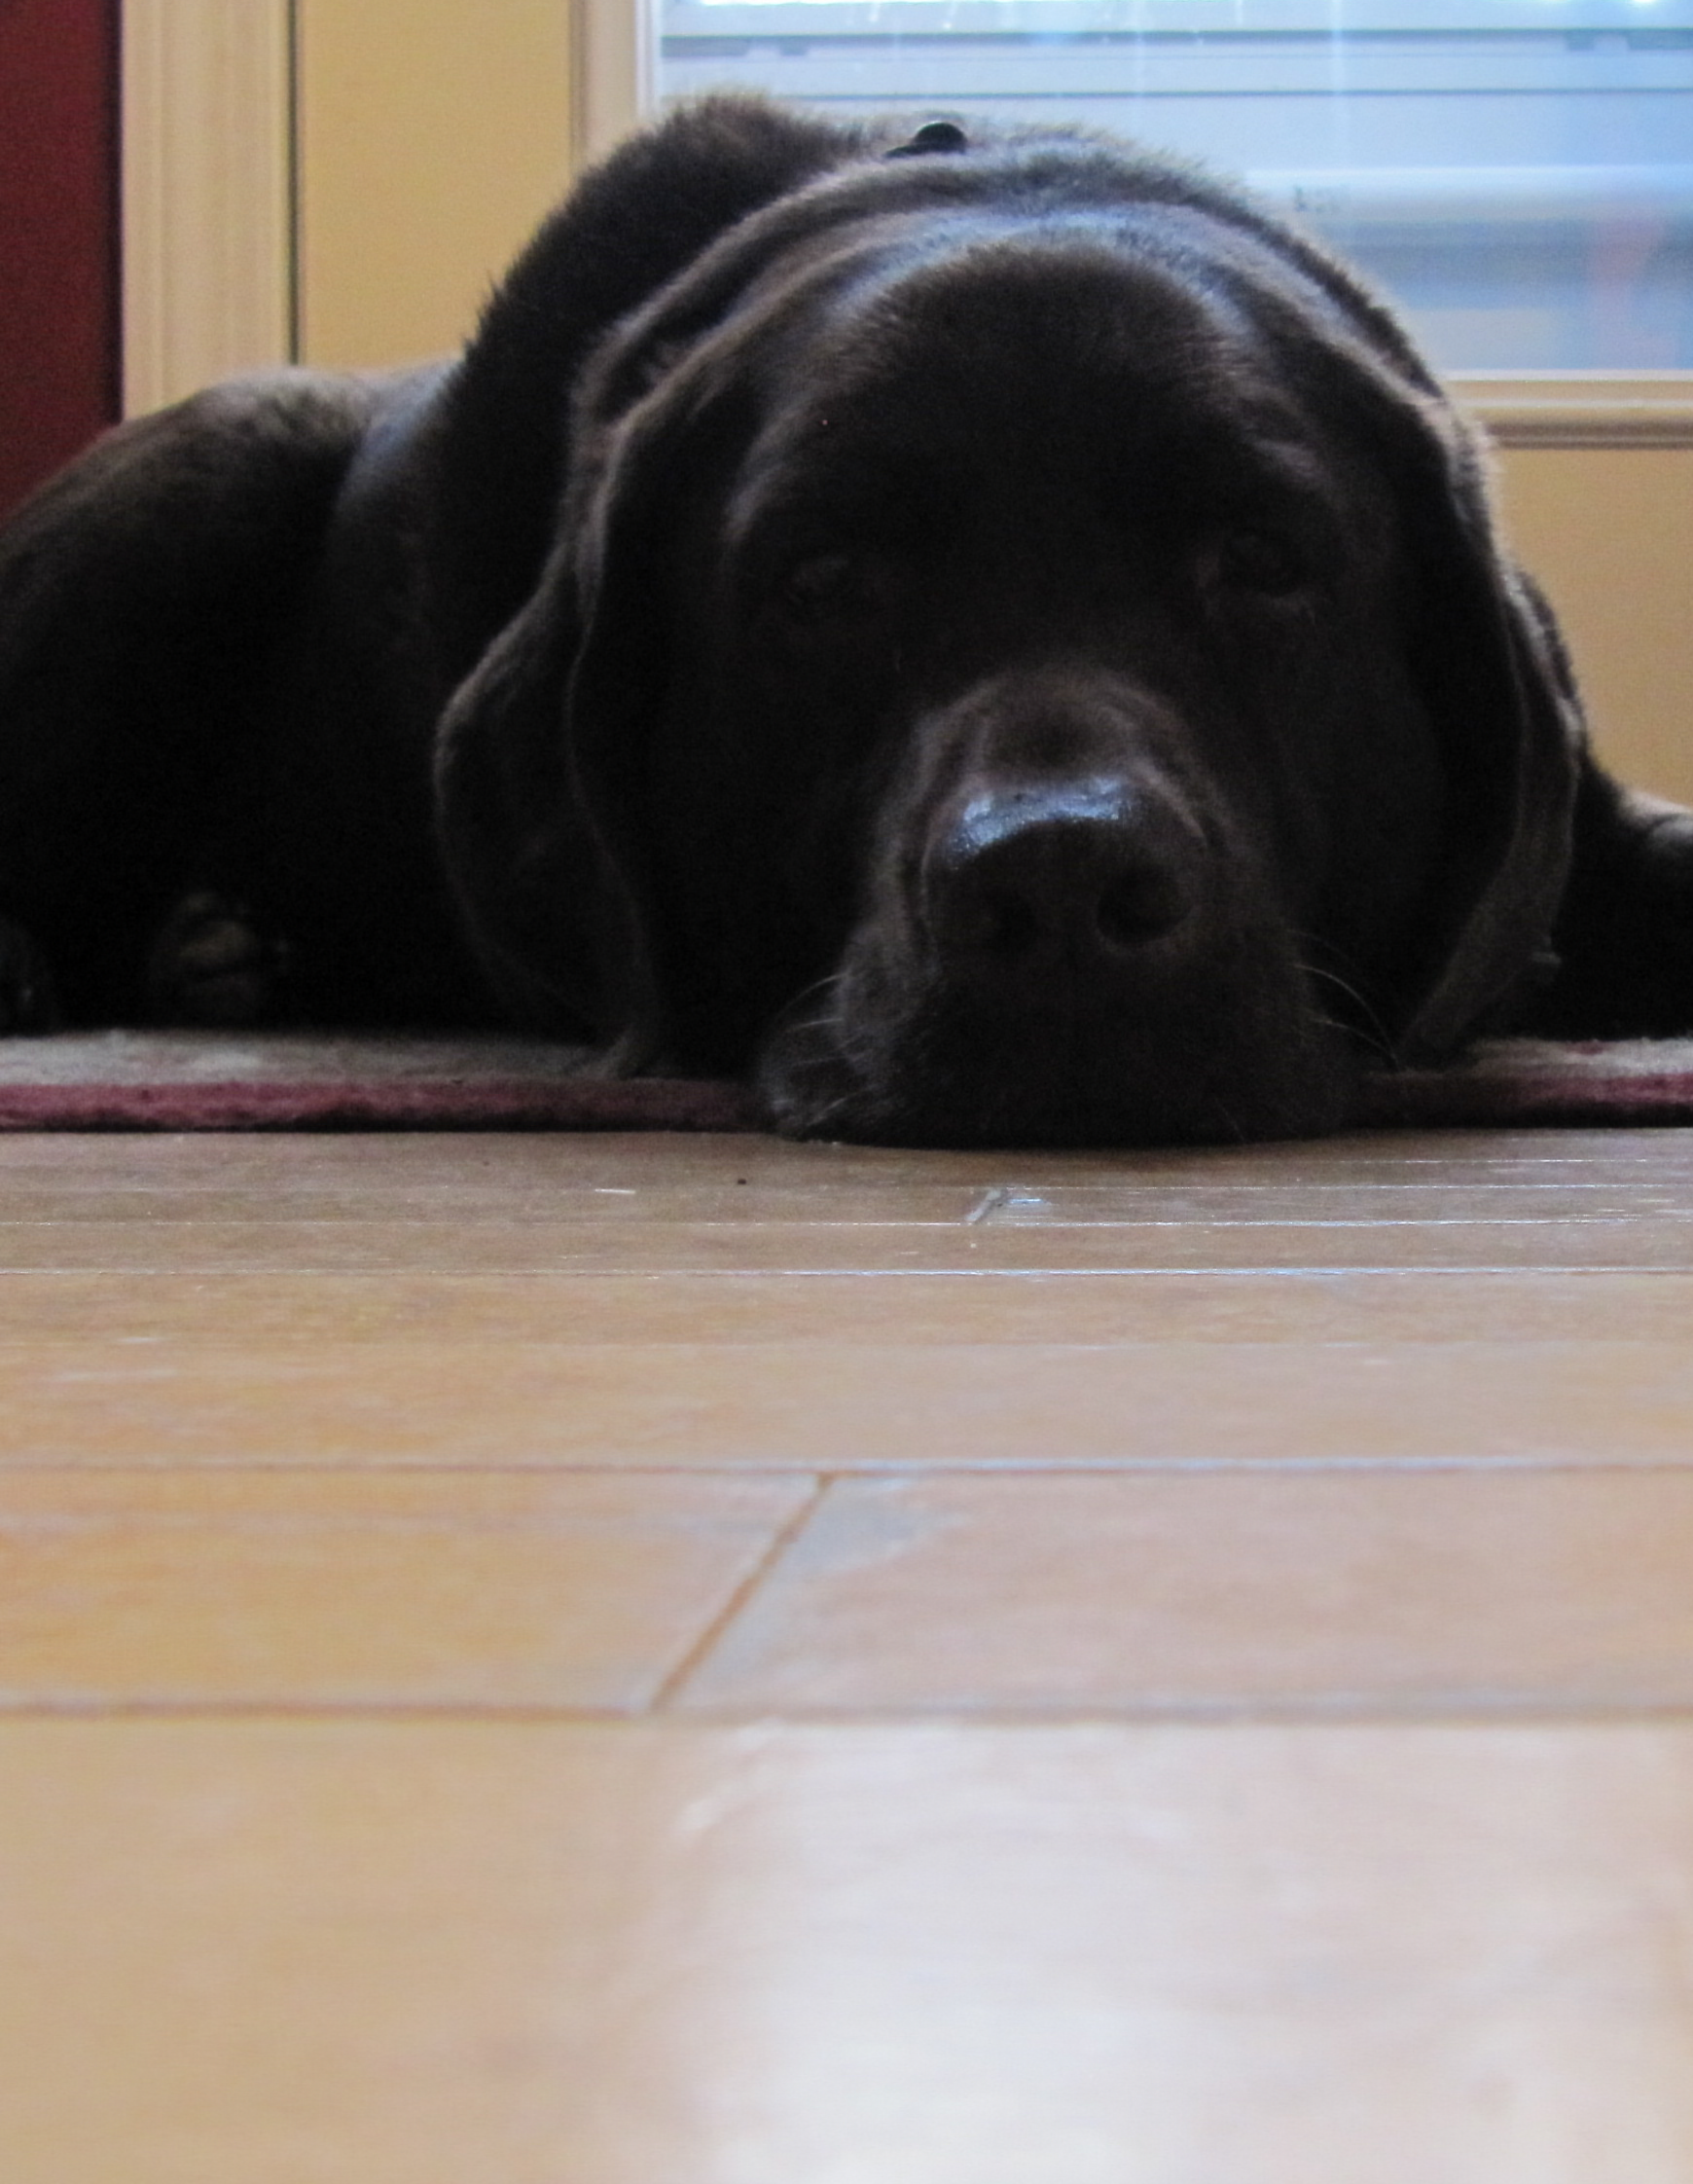
\includegraphics[width=.4\textwidth]{pix/suzy_cover_squeezed.png}}
\end{center}
(The top singular value is 
$291533.51$.
% $39038.59$,
% $30526.84$,
% $19983.01$,
% $13946.40$,
% $11523.07$,
% $9354.02$, and
% $8067.98$.
The twenty percent cutoff is $129.23$. 
The smallest of the $1739$ singular values is $3.36$.)
The picture on the left is $4$~megabytes, 
while the right is~$3.4$.


\section{Source of plot\_action.sage}

The \inlinecode{plot_circle_action}
routine takes the four entries of the $\nbyn{2}$
matrix and returns a list of two graphics, showing the input and the
output.
Other parameters are the number of colors and a flag giving whether
to plot a full circle or just the top half circle.

The driver routine computes the list of colors and 
calls a helper \inlinecode{color_circle_list}, 
given below, which returns a list of graphics.
Finally, the routine plots those graphics.
\lstinputlisting[firstline=39,lastline=50]{plot_action.sage}

The helper routine does the heavy lifting.
There are two global values to set graphic values.
The variable \inlinecode{CIRCLE_THICKNESS} sets the thickness of 
the plotted curve, in points (a printer's unit, here $1/72$~inch).
Similarly \inlinecode{DOT_SIZE} sets the size of the small empty circle.
This routine produces a parametrized curve $(x(t),y(t))$ and uses \Sage's
\inlinecode{parametric_plot} function to get the resulting graphic.
\lstinputlisting[firstline=5,lastline=36]{plot_action.sage}
If this routine is plotting the upper half circle then it adds the
small empty circle at the end to show that the image of $(-1,0)$
is not part of the graph.




\section{Source of img\_squeeze.sage}
We use the Python Image Library for reading and writing the graphic.
\lstinputlisting[firstline=5,lastline=5]{img_squeeze.sage}
The function
\inlinecode{img_squeeze}
takes three arguments:~the names of the two files, and
the cutoff real number between $0$ and~$1$ the gives the percentage 
of the singular values to retain in the sum.
\lstinputlisting[firstline=7,lastline=11]{img_squeeze.sage}

This function first brings the input data to a format where each
pixel is a triple 
$(\text{red}, \text{green},\text{blue})$ of integers that range from 
$0$ to~$255$.
It uses those numbers to build 
three Python arrays \inlinecode{rd}, \inlinecode{gr},
and \inlinecode{bl}, which then initialize the 
three \Sage{} matrices \inlinecode{RD},
\inlinecode{GR}, and~\inlinecode{BL}.
\lstinputlisting[firstline=12,lastline=28]{img_squeeze.sage}

The next step finds the Singular Value Decomposition of those three.
Out of curiosity, we have a look at the eight largest singular
values in the red matrix, the singular value where we make the cutoff,
and the eight smallest.
\lstinputlisting[firstline=29,lastline=40]{img_squeeze.sage}

Finally, for each matrix we compute the sum
$\sigma_1\cdot\vec{u}_1\trans{\vec{v}}_1+\sigma_2\cdot\vec{u}_2\trans{\vec{v}}_2
   +\cdots$
up through the cutoff index.
\lstinputlisting[firstline=41,lastline=60]{img_squeeze.sage}

To finish, we put the data in the PNG format and save it to 
disk.
\lstinputlisting[firstline=61,lastline=69]{img_squeeze.sage}
This part of the routine takes a long time, in part because
the code is intended to be easy to read rather than fast to run.

\endinput


TODO:
1) mention Sage matrices are not mutable in matrix introduction.
Is mutable discussed in Intro?

2) vectors have to be forced to be row or col

2) Need int() fcns?  copy() fcn?